\chapter{Avalia\c{c}\~{a}o Experimental} \label{chap:avaliacao}
A realização do monitoramento dos sinais motores, de uma maneira não invasiva, é um desafio. Logo, esta tese fornece uma forma lúdica de monitorar os dados de saúde, por meio de jogos eletrônicos que podem ser integrados à rotina diária dos usuários. Neste capítulo, iremos demonstrar que conseguimos desenvolver um~\ac{sms} não invasivo para monitoramento de um sinal do~\ac{dp} com uma taxa de acurácia de 86,67\%.




\section{ETAPA 1 - Entrevista Semiestruturada com Profissionais de Saúde}\label{sec:entrevista_semi_estruturada}



A interpretação de dados é o cerne da pesquisa qualitativa, tem como função desenvolver a teoria e servir, ao mesmo tempo, de base para a decisão sobre quais dados adicionais devem ser coletados, por meio de codificação seletiva~\cite{FLI04}. Esta técnica permite elaborar uma categorização nos dados e demonstrar ao pesquisador quais são os fenômenos mais preponderantes da pesquisa. O procedimento da interpretação dos dados, assim como a integração de material adicional, são encerrados quando se atinge a ``saturação teórica'', ou seja, quando o avanço na codificação não resulta na aquisição de novos conhecimentos~\cite{FLI04}.

Para análise dos textos provenientes da pesquisa, foram transcritas as entrevistas com neurologistas e fisioterapeutas especialistas em neurologia. Com  a codificação seletiva, foi possível categorizar as ocorrências de acordo com o conteúdo de cada texto. Ou seja, as respostas de cada participante foram analisadas e incluídas na árvore de categorias como sugere o método de pesquisa~\cite{FLI04}. 

Para auxiliar no processo de análise, seleção e codificação, foi utilizada uma ferramenta de suporte à pesquisa qualitativa (\textit{QDA Miner}~\cite{qda13}) e, por meio desta, foi possível categorizar e reformular a árvore de categorias~\cite{FLI04} diversas vezes durante o processo de análise~\cite{FLI04}.


\subsection{Objetivo da Entrevista Semiestruturada}
O objetivo da entrevista semiestruturada~\cite{FLI04} foi entender como é feito o acompanhamento do paciente com sintomatologia do~\ac{dp}, juntamente aos profissionais de saúde: neurologistas, que prescrevem a dosagem medicamentosa, e fisioterapeutas, que fazem o tratamento de reabilitação e acompanhamento motor do paciente. Esses profissionais de saúde foram indagados se haveria melhora na tomada de decisão, caso estes pudessem acompanhar os sinais motores diariamente. Procurou-se encontrar, dentro do contexto de estudo, a importância do monitoramento de dados de saúde e os benefícios trazidos por este.

As entrevistas foram realizadas presencialmente, com perguntas não estruturadas e com uma maior estruturação no decorrer da entrevista, preocupando-se em evitar a referência do entrevistador sobre os pontos de vista do entrevistado, conforme sugere o método científico~\cite{FLI04}. 

\subsubsection{Instrumento de Análise dos Dados da Pesquisa Qualitativa} \label{section:analise_dados} 
A pesquisa qualitativa assistida por computador permite uma melhor categorização das informações obtidas em modo texto. O software QDA Miner~\cite{qda13} auxilia o pesquisador na organização dos registros da pesquisa e em suas interpretações, justificando-se o uso da ferramenta devido à dificuldade de classificar e analisar os dados obtidos. Nessa análise, foram consideradas as atividades referentes ao acompanhamento dos sinais motores em pacientes com~\ac{dp}. Buscou-se, durante a pesquisa, avaliar se um cenário de monitoramento dos sinais motores, por meio de jogos eletrônicos, auxiliaria os profissionais de saúde quanto ao tratamento de seus pacientes.

Nesta seção, faz-se um detalhamento do resultado da entrevista semiestruturada, que descreve a opinião dos entrevistados, e coleta-se requisitos baseados em suas necessidades, devidamente expostas. Por meio desta entrevista, foi avaliada a \textbf{ETAPA 1}: \textit{Quais os benefícios de acompanhar os sinais motores do paciente diariamente, do ponto de vista do profissional da saúde?}




\subsection{Perfil dos Participantes}
O perfil dos participantes é composto por quatro profissionais da saúde, dos quais dois são fisioterapeutas, com especialização em neurologia, e dois são médicos neurologistas. A escolha desse perfil se fez de acordo com seus ofícios, responsabilidades e complementaridade quanto ao tratamento do paciente. Os neurologistas realizam o diagnóstico e acompanham os sinais motores juntamente com as informações obtidas do paciente ou de seu cuidador, e, baseados nestas informações, realizam o gerenciamento da dosagem medicamentosa da doença. Por outro lado, os fisioterapeutas fazem o acompanhamento dos sinais motores em sessões de fisioterapia e promovem a reaprendizagem motora destes pacientes. Logo, esses profissionais possuem visões e preocupações distintas, inerentes ao seu ofício. 

Para manter a confidencialidade de informação, os entrevistados receberam uma \textbf{LEGENDA}, que identifica o perfil profissional seguido por um número sequencial, o qual identifica o entrevistado, mas preserva sua identidade (Tabela~\ref{table:perfil_analise_participantes}).

\begin{table}[h]
\caption{Perfil dos Participantes}
\label{table:perfil_analise_participantes}
\begin{tabular}{|l|l|c|c|}
\hline
\textbf{LEGENDA} & \textbf{PROFISSÃO}             & \multicolumn{1}{|l}{\textbf{IDADE (ANOS)}} & \multicolumn{1}{|l|}{\textbf{EXPERIÊNCIA (ANOS)}} \\ \hline
FIS\_01          & Fisioterapia em Neurologia & 40                                         & 10                                                \\ \hline
FIS\_02          & Fisioterapia em Neurologia     & 39                                         & 10                                                \\ \hline
NEU\_01          & Médico Neurologista            & 42                                         & 15                                                \\ \hline
NEU\_02          & Médico Neurologista            & 67                                         & 30                                                \\ \hline
\end{tabular}

\end{table}

\subsubsection{Questionário de Pesquisa}
Para a formulação do questionário, foram realizadas análises nas diretrizes médicas~\cite{protpar010,national2006parkinson} e na tabela UPDRS~\cite{updrs87}, sobre o progresso do~\ac{dp} e dos sinais monitoráveis por sensores de movimento. Para a entrevista, foram elaboradas 15 perguntas, agrupadas em 3 seções (Apêndice \ref{apendice:entrevista-semi-estruturada}), com os seguintes temas: sinais do~\ac{dp}, monitoramento da saúde motora e benefícios advindos do monitoramento. O entrevistador selecionou as questões de acordo com o perfil profissional.

\subsection{Análise}
Durante a análise das entrevistas, foram extraídos fragmentos, e a nomenclatura utilizada contém o prefixo \textbf{FRAGMENTO} mais um número sequencial identificando-o. Esse procedimento permite identificar \textbf{requisitos} que orientem a proposta de monitoramento de dados motores por intermédio de jogos eletrônicos. Logo, os requisitos extraídos nesta abordagem foram obtidos a partir da perspectiva do profissional de saúde em relação ao tratamento e ao acompanhamento do~\ac{dp}. 

\subsubsection{Diagnóstico}\label{section:analise_diagnostico}

Na entrevista junto aos neurologistas, foi indagado como o diagnostico do~\ac{dp} é realizado.  A entrevista corroborou com a literatura médica~\cite{tolosa06,vedolin2003} em relação ao diagnóstico de exclusão do \ac{dp}~\cite{protpar010,national2006parkinson}.  

Todos os profissionais informaram que o sintoma mais comum é o tremor de repouso, e que este é inicialmente unilateral, seguido de uma bradicinesia, como podemos perceber nos fragmentos ([FRAGMENTO-01], FRAGMENTO-02]). Ainda no ([FRAGMENTO-01]), existe uma ocorrência do \textbf{[NEU\_01]}, em que o mesmo evoca sobre a importância da técnica de \textit{Finger Taps} ~\cite{updrs87} para avaliação da bradicinesia.




\begin{quote}
\textbf{[FRAGMENTO-01][NEU\_01]} - 
\emph{
O diagnóstico da doença de Parkinson é dado, principalmente, quando o paciente chega se queixando de tremor. Esse sintoma começa com um tremor unilateral, geralmente, pelas mãos, lentamente progressivo e de repouso. Além do tremor, esse paciente exibe uma lentidão que detectamos pelo \textit{Finger Taps}. Essa técnica consiste em tocar o polegar no primeiro e no segundo dedo simultaneamente, para ver se há ou não lentidão. Faz-se uma comparação sempre com o outro lado para visualizar possíveis diferenças. Existe, também, uma rigidez no braço, quando faz-se uma flexão e extensão do membro e percebe-se que o tônus desse paciente, comparado com o outro lado, exibe uma diferença.
}
\end{quote}

\begin{quote}
\textbf{[FRAGMENTO-02][NEU\_02]} -
\emph{
O diagnóstico da doença de Parkinson é feito com uma das queixas iniciais do paciente: o tremor de repouso, associado  a dificuldade na marcha. Então, normalmente, os pacientes reclamam de uma perna presa e um tremor de repouso. 
}
\end{quote}

Uma ocorrência no ([FRAGMENTO-03]) que deve ser ressaltada é o que o entrevistado referiu como ``\textit{boa resposta ao prolopa}''. Essa ocorrência é denominada de diagnóstico diferencial do~\ac{dp} ~\cite{protpar010} e consiste na redução dos sinais parkinsonianos em decorrência da resposta ao tratamento medicamentoso. 

\begin{quote}
\textbf{[FRAGMENTO-03][NEU\_01]} - 
\emph{
Então, os sinais são: o tremor em repouso, lentidão e a rigidez. Apenas de um lado inicialmente, por exemplo, começa no braço direito e depois vai para a perna direita, depois para o braço esquerdo e depois a perna esquerda. Isso lentamente progressivo, fazemos a exclusão com outras doenças através de outros exames, como tomografia, ressonância ou uma boa resposta ao prolopa.
}
\end{quote}

\subsubsection{Sintomas}
Nesta seção, estão expostos sinais para o acompanhamento da sintomatologia do~\ac{dp}.

O sintoma de tremor, além de ter sido referenciado durante o diagnóstico da doença, na Seção ~\ref{section:analise_diagnostico}, por todos os entrevistados, possui particularidades, como a dificuldade de controlar o sintoma por intermédio do tratamento medicamentoso ([FRAGMENTO-04]), e não é tão incapacitante quanto a bradicinesia. No ([FRAGMENTO-05]), o [NEU\_01] reforçou sobre a importância de controlar os sinais de lentidão do movimento ante os de tremor~\cite{do2007parkinson}.

\begin{quote}
\textbf{[FRAGMENTO-04][NEU\_01]} - 
\emph{
Necessário observar porque o tremor é, as vezes, mais difícil de controlar, pois está relacionado ao emocional do paciente e, quanto mais emocionalmente desequilibrado o paciente tiver, mais tremor ele tem.
}
\end{quote}

\begin{quote}
\textbf{[FRAGMENTO-05][NEU\_01]} - 
\emph{
O controle do tremor é um pouco complicado, devido a dificuldade dominá-lo com as medicações existentes hoje. Então, você poderia ver nesse seu projeto a lentidão. Porque, o paciente poderá apresentar lentidão, porém o paciente quer tremer, mas não quer ficar lento.
}
\end{quote}


O pesquisador indagou se o sintoma da bradicinesia era considerado o mais debilitante do~\ac{dp}; como resposta, ele obteve a afirmação de que a bradicinesia impacta, diretamente, na qualidade de vida do paciente, privando-o de realizar atividades diárias ([FRAGMENTO-06]).

\begin{quote}
\textbf{[FRAGMENTO-06][NEU\_01]} - 
\emph{
É ele atrapalha né, principalmente no levantar, andar. Para você se levantar, pentear o cabelo, o tremor é prejudicial. Porém, mais prejudicial ainda, é a lentidão do movimento.
}
\end{quote}

Ao indagar se o movimento de adução e abdução do braço seria relevante para a identificação do~\ac{dp}, o [NEU\_01] informou que a bradicinesia é um sintoma que traz lentidão em todo o corpo e, possivelmente, seria afetada por este movimento, pois, devido à redução dos movimentos automáticos ([FRAGMENTO-07]), traz outros impactos físicos ao paciente ([FRAGMENTO-08]).

\begin{quote}
\textbf{[FRAGMENTO-07][NEU\_01]} - 
\emph{
Na verdade, o movimento da abdução demonstrará o quão lento está. Porque, o comprometimento na doença de Parkinson está no comprometimento piramidal. O comprometimento extra-piramidal não vai estar alterando a força motora. No entanto, o comprometimento piramidal irá impactar justamente na lentidão. Por exemplo, quando um paciente com~\ac{dp} está andando, percebe-se a redução dos movimentos automáticos, principalmente, no balançar dos braços. Ele vai andando, vai andando, e você percebe que o paciente que está com a força e com a estrutura piramidal normal. No entanto, anda lento em consequência da redução dos movimentos automáticos.
}
\end{quote}


\begin{quote}
\textbf{[FRAGMENTO-08][FIS\_01]} - 
\emph{
Os sinais mais frequentes a gente tem a bradicinesia que é a lentificação do movimento, a gente tem um padrão postural que começa a ficar bem nítido que o paciente apresentar o Parkinson. Você percebe uma perda da movimentação automática da cintura escapular e aí ele começa a apresentar uma diminuição no volume da voz que é uma diplofonia, e apresenta uma maior rigidez muscular. Eles reclamam bastante e a bradicinesia que tornam os movimentos cada vez mais lentos.
}
\end{quote}




\subsubsection{Monitoramento Motor}
Nesta seção, está exposta a importância do monitoramento dos sinais capturados no estudo analítico de caso controle, definido no método de pesquisa na Seção~\ref{section:estudo_caso_controle}. Nesse estudo, também pretende-se identificar as características dos movimentos que possam ser extraídos desses sinais, e que venham fornecer subsídios para diferenciar indivíduos diagnosticados com~\ac{dp} ante indivíduos sem o diagnóstico.

Ao indagar ao [FIS\_02] se o movimento de adução e abdução do braço seria relevante para a identificação do~\ac{dp}, este informou que mesmo não sendo um teste específico para a identificação da doença, existem diferenças significativas encontradas em indivíduos diagnosticados com parkinson [FRAGMENTO-11].
\begin{quote}
\textbf{[FRAGMENTO-11][FIS\_02]}-
\emph{
Sim. Existe alterações sim, mas eu nunca vi especificamente esse teste como sendo usado para diagnóstico da doença. Mas que realmente existem mudanças no movimento de adução e abdução de uma pessoa normal ante a um parkinsoniano.
}
\end{quote}

O [FIS\_01] explicou os motivos que levam a perda da mobilidade no movimento de adução e abdução ([FRAGMENTO-12]) e, consequentemente, reforça que esse movimento poderia ser monitorado para verificar o comprometimento da doença. Em um outro fragmento ([FRAGMENTO-13]), o mesmo fisioterapeuta menciona a importância de monitorar a amplitude do movimento, pois permite visualizar a resposta do paciente ao tratamento oferecido.

\begin{quote}
\textbf{[FRAGMENTO-12][FIS\_01]}-
\emph{
Têm, porque uma das grandes perdas que eles apresentam é na cintura escapular e consequentemente é pegando a parte de ombro. Pois caso ela seja mais fixa, porque geralmente o paciente de Parkinson abduz o ombro. O ombro fica abduzido junto ao tronco e ai ele perde a mobilidade do cotovelo e punho e também o movimento fica comprometido por conta disso.
}
\end{quote}

\begin{quote}
\textbf{[FRAGMENTO-13][FIS\_01]}-
\emph{
Mesmo sabendo que a tendência é uma lentificação (bradicinesia).  As outras doenças também, porque um dos objetivos nossos é o aumento da amplitude. Então é um meio interessante para a gente conseguir visualizar se o tratamento está dando certo ou não.
}
\end{quote}



\subsubsection{Velocidade do Movimento De Adução e Abdução dos Braços}
Um ponto de convergência entre os profissionais entrevistados é a importância de monitorar a velocidade angular dos pacientes. Os profissionais tentam associar o tratamento fisioterápico e medicamentoso para a melhora da bradicinesia. Logo, para estes profissionais, a melhora está condicionada a um aumento na velocidade do movimento ([FRAGMENTO-14],[FRAGMENTO-15])

\begin{quote}
\textbf{[FRAGMENTO-14][NEU\_01]} - 
\emph{
É como eu falei para mim seria melhor se capturássemos se ele está mais lento. Se através dessa amplitude você conseguir por intermédio do computador identificar que ele está mais lento de um lado do que do outro, e conseguir visualizar a velocidade de um lado e do outro. Então isso é interessante.
}
\end{quote}


\begin{quote}
\textbf{[FRAGMENTO-15][FIS\_01]} - 
\emph{
É e consequentemente a velocidade, porque nesse caso o tratamento é diretamente relacionado a isso quanto mais veloz o parkinsoniano é melhor para a gente melhor prognóstico a gente pode ter lá na frente. Mesmo sabendo que a tendência é uma lentificação.
}
\end{quote}


A assimetria do movimento acomete os pacientes que estão nos estágios iniciais da doença. Por esse motivo, geralmente ela é identificada durante o diagnóstico [FRAGMENTO-03]. Porém, alguns pacientes parkinsonianos apresentam a assimetria do movimento quando um dos lados é mais comprometido que o outro. Por essa razão é que o [NEU\_01] afirmou: \textit{``Se através dessa amplitude você conseguir por intermédio do computador identificar que ele está mais lento de um lado do que do outro''}. Pois, a tendência natural da evolução do~\ac{dp} é a redução na assimetria do movimento conforme a opinião do [NEU\_01] no [FRAGMENTO-16] e na tabela UPDRS ~\cite{updrs87} em sua escala de avaliação do progresso da doença (Seção ~\ref{section:escalas_avaliacao}).

\begin{quote}
\textbf{[FRAGMENTO-16][NEU\_01]}-
\emph{
No início. Geralmente o paciente se queixa de uma diminuição de força de um lado do corpo. Mas na progressão, ele vai sentir dificuldade global. Mas aqueles parkinsonianos iniciais geralmente eles se queixam na diminuição do movimento de um dos lados.
}
\end{quote}

\subsubsection{Benefícios Advindos do Monitoramento}


Em relação aos benefícios advindo do monitoramento pudemos identificar a quantificação dos sinais motores, a amplitude de movimento de adução e abdução do braço e a velocidade angular destes movimentos. Essa análise trouxe dois grupos de respostas: o primeiro reconhecia a importância da quantificação dos dados para identificar a melhora ou piora do paciente [FRAGMENTO-17], e o outro relatava que essa informação tinha mais validade científica do que prática [FRAGMENTO-18]. Todavia, caso esses profissionais tivessem acesso a um sistema que permitisse o monitoramento motor, possivelmente eles iriam perceber os benefícios da abordagem e modificar sua prática atual ao adotar uma nova proposta.

\begin{quote}
\textbf{[FRAGMENTO-17][FIS\_02]}-
\emph{
É preciso ter parâmetros sim. Pois atualmente usamos muito o olho clínico e ai vai de cada profissional. Se tivermos números facilitam bastante porque se tornam fatos e basearmos nossas conclusões em números é bem melhor.
}
\end{quote}

\begin{quote}
\textbf{[FRAGMENTO-18][FIS\_01]}-
\emph{
É interessante em termos de pesquisa. Em termos de clínica a geralmente a gente vai no geral. Por exemplo: Eu faço uma flexão de ombro com bastão e anotei no meu exame que ele ia até mais ou menos 70º e após 15 dias eu vejo que ele está levantando acima de 90º. Então está marcado a minha evolução. Então eu faço a avaliação nesse sentido. Então esse sistema seria bom para pesquisa mesmo.
}
\end{quote}


Indagou-se aos profissionais se o monitoramento dos sinais motores auxiliaria no gerenciamento da dosagem medicamentosa. Os profissionais informaram que sentem a necessidade de visualizar a eficácia do tratamento diante do paciente. O [FIS\_01], no [FRAGMENTO-19], cita a importância de avaliar tanto o tratamento medicamentoso quanto se a sua atividade fisioterápica traz benefícios ao paciente. Os neurologistas ([NEU\_01] e [NEU\_01]) citam a importância de reajustar a dosagem medicamentosa e que a quantificação do sintoma identifica o resultado do efeito medicamentoso. Outra opinião bastante pertinente é que o agravamento do~\ac{dp} é bastante sutil do ponto de vista do [NEU\_01], no [FRAGMENTO-21]. Logo, se for possível mostrar a evolução da doença em períodos mais longos, o tratamento seria mais efetivo e, consequentemente, traria uma melhor qualidade de vida aos pacientes.

\begin{quote}
\textbf{[FRAGMENTO-19][FIS\_01]} - 
\emph{
 É interessante porque teremos uma ideia de até que ponto a medicação está sendo efetiva, até quando a patologia está progredindo e também avaliar se o nosso tratamento fisioterápico está dando resultados ao tentar frear a evolução da doença.
}
\end{quote}


\begin{quote}
\textbf{[FRAGMENTO-20][NEU\_02]} - 
\emph{
Sim. Dentro do que você propõe. Com certeza sim. Essa avaliação desses movimentos. Porque a gente consegue visualizar se a medicação está surtindo efeito, se precisa ser reajustada.
}
\end{quote}

\begin{quote}
\textbf{[FRAGMENTO-21][NEU\_01]} - 
\emph{
Se esse mecanismo acontecesse. Você poderia avaliar a dosagem de um paciente por exemplo. Veja avalie durante uma semana, não melhorou. Então a gente poderia fazer um teste com tremor, lentidão e a rigidez, se houvesse esse aspecto.  A gente poderia aumentar a dosagem e visualizaria a eficácia da dosagem com o decorrer do tempo, com o decorrer da evolução. E verificaria se realmente o paciente está melhorando. Porque o paciente da doença de Parkinson ele piora lentamente, as vezes é tão sutil que o próprio paciente não consegue. Então é como eu disse, cada paciente a evolução é diferente num existe. Mas poderia assim, se você conseguisse detectar as amplitudes do tremor por exemplo.
}
\end{quote}


\subsection{Requisitos Identificados}
A \ac{er} é o processo de descobrir o propósito do software, identificando os principais envolvidos do sistema com suas respectivas necessidades e documentando a análise para uma implementação posterior \cite{bas00}. Contudo, é um processo que deve ser continuamente repetido para que as necessidades dos envolvidos sejam satisfeitas. As técnicas para identificação de requisitos são derivadas principalmente das ciências sociais, que se baseiam em pesquisa qualitativa na qual são analisadas a teoria do objeto de estudo e a experiência prática dos envolvidos na pesquisa ~\cite{elicquest05,zowghi2005}.

A identificação dos requisitos de um sistema representa o início da elicitação das necessidades da solução proposta. Então, os requisitos definem quais serão os serviços que o sistema deve prover além de um conjunto de restrições existentes na sua operação~\cite{sommerville2011}. A técnica utilizada para a identificação dos requisitos desta pesquisa é baseada em pesquisa qualitativa, em que se usou a entrevista semiestruturada, na qual o entrevistador possui um conjunto de perguntas pré-definidas e guia a entrevista de acordo com a opinião do entrevistado~\cite{FLI04}.

Ficou definido que cada requisito deve ser importante para os entrevistados, e a nomenclatura estabelecida é de \textbf{REQ-ENTREVISTAS} seguida por um número sequencial correspondente à sua apresentação. Para demonstrar a relevância dos requisitos, a teoria foi confrontada com o que é aplicado na prática pelos profissionais de saúde; por esse motivo, foram citadas referências científicas que corroboram com a análise. 

\begin{description}
	\item[REQ-ENTREVISTAS-01:] Identificar e quantificar o tremor parkinsoniano~\cite{tolosa06,keijsers2006,lemoyne2010}.
	\item[REQ-ENTREVISTAS-02:] Identificar a bradicinesia~\cite{patel_monitoring_2009}. 
	\item[REQ-ENTREVISTAS-03:] Avaliar bradicinesia usando~\textit{finger-tapping}~\cite{finger2012}.
	\item[REQ-ENTREVISTAS-04:] Considerar e identificar a assimetria do movimento nos estágios iniciais~\cite{national2006parkinson}.	
	\item[REQ-ENTREVISTAS-05:] Fornecer mecanismos para possibilitar o Diagnóstico Diferencial~\cite{protpar010} da Doença de Parkinson. 
	\item[REQ-ENTREVISTAS-06:] Analisar a Marcha~\cite{gaitusingsensorsreview2012}. Medir a marcha e comparar o padrão do movimento com indivíduos com e sem o diagnóstico do~\ac{dp} para classificar a marcha como saudável ou parkinsoniana.
	\item[REQ-ENTREVISTAS-07:] Calcular e armazenar a amplitude do movimento de adução e abdução dos braços, para realizar o monitoramento da saúde motora e poder acompanhar o tratamento.
	\item[REQ-ENTREVISTAS-08:] Calcular e armazenar a velocidade angular do movimento de adução e abdução dos braços. Para poder avaliar o sintoma da bradicinesia.
	\item[REQ-ENTREVISTAS-09:] Avaliar estado emocional baseado na ocorrência e comprometimento do tremor. 
\end{description}



\subsubsection{Inviabilidade Técnica}
Alguns requisitos identificados não podem ser implementados com a tecnologia de sensor de movimento usada nesse trabalho. A importância destes requisitos é reconhecida e pode ser implementada em trabalhos futuros, desde que as barreiras tecnológicas sejam resolvidas, como definido a seguir:

	\begin{figure}[!ht]
	\centering
	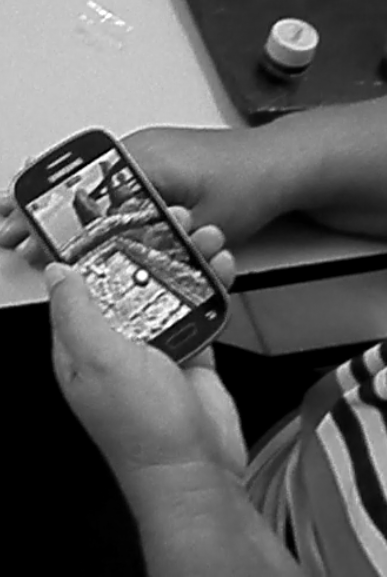
\includegraphics[scale=0.5]{./img/gametremor.png}
	\caption{Teste de um jogo usando acelerômetro para quantificação do sinal de tremor do Parkinson}
	\label{fig:gametremor}
	\end{figure}

\begin{itemize}
	\item O \textbf{REQ-ENTREVISTAS-01} não foi possível, pois o tremor de repouso é um dos principais sinais do~\ac{dp}. Sabíamos da sua importância, inclusive foi desenvolvido um jogo para \textit{Smartphone} que pudesse quantificar o tremor (Figura ~\ref{fig:gametremor}). Porém, no teste junto aos usuários, foi percebido que, no momento do uso, os pacientes com~\ac{dp} cessavam o tremor, inviabilizando assim sua quantificação. 
	\item O \textbf{[REQ-ENTREVISTAS-03]} não foi possível, pois a técnica de \textit{finger-tapping} não pode ser avaliadas utilizando o MS-Kinnect 1.0, uma vez que nessa versão não existe a captura do movimento dos dedos, conforme ilustrado na Figura~\ref{fig:articulacoeskinnect}.
	\item O \textbf{REQ-ENTREVISTAS-09} não foi possível, pois, por envolver estado emocional e parâmetros que não estamos levando em consideração nesse trabalho, esse requisito está fora do escopo. Entretanto, com mecanismos de detecção de batimentos cardíacos presente no MS-Kinnect 2.0, pode ser averiguada a relação dos batimentos cardíacos com o tremor.
\end{itemize}




\subsubsection{Matriz de Rastreabilidade - Fragmento x Requisitos}

\begin{table}[!htb]
\caption{Matriz Rastreabilidade: Fragmento x Requisitos}
\label{table:matrix_rastreabilidade}
\begin{tabular}{||p{6.06cm}||ccccccccc|}
\hline
 \multicolumn{1}{|p{6.06cm}|}{\centering \textbf{FRAGMENTOS / REQUISITOS}} &  01 &  02 &  03 &  04 &  05 &  06 &  07 &  08 & 09 \\ 
\hline 
 \multicolumn{1}{|p{6.06cm}|}{\centering 01} &  x &  x &  x &  x &   &   &   &   &  \\ 
 \multicolumn{1}{|p{6.06cm}|}{\centering 02} &  x &   &   &   &   &  x &   &   &  \\ 
 \multicolumn{1}{|p{6.06cm}|}{\centering 03} &  x &  x &   &  x &  x &   &   &   &  \\ 
 \multicolumn{1}{|p{6.06cm}|}{\centering 04} &  x &   &   &   &   &   &   &   & x \\ 
 \multicolumn{1}{|p{6.06cm}|}{\centering 05} &  x &  x &   &   &   &   &   &   &  \\ 
 \multicolumn{1}{|p{6.06cm}|}{\centering 06} &   &  x &   &   &   &  x &   &   &  \\ 
 \multicolumn{1}{|p{6.06cm}|}{\centering 07} &   &  x &   &   &   &  x &  x &  x &  \\ 
 \multicolumn{1}{|p{6.06cm}|}{\centering 08} &   &  x &   &   &   &  x &  x &  x &  \\ 
 \multicolumn{1}{|p{6.06cm}|}{\centering 09} &   &   &   &  x &   &  x &   &   &  \\ 
 \multicolumn{1}{|p{6.06cm}|}{\centering 10} &   &   &   &   &   &  x &   &   &  \\ 
 \multicolumn{1}{|p{6.06cm}|}{\centering 11} &   &   &   &   &   &   &  x &   &  \\ 
 \multicolumn{1}{|p{6.06cm}|}{\centering 12} &   &  x &   &   &   &   &  x &  x &  \\ 
 \multicolumn{1}{|p{6.06cm}|}{\centering 13} &   &   &   &   &   &   &  x &   &  \\ 
 \multicolumn{1}{|p{6.06cm}|}{\centering 14} &   &  x &   &   &   &   &   &   &  \\ 
 \multicolumn{1}{|p{6.06cm}|}{\centering 15} &   &  x &   &  x &   &   &   &  x &  \\ 
 \multicolumn{1}{|p{6.06cm}|}{\centering 16} &   &   &   &  x &   &   &   &   &  \\ 
 \multicolumn{1}{|p{6.06cm}|}{\centering 17} &   &   &   &   &   &   &   &   &  \\ 
 \multicolumn{1}{|p{6.06cm}|}{\centering 18} &  x &   &  x &  x &   &  x &  x &  x & x \\ 
 \multicolumn{1}{|p{6.06cm}|}{\centering 19} &  x &   &   &   &  x &  x &  x &  x &  \\ 
 \multicolumn{1}{|p{6.06cm}|}{\centering 20} &  x &   &   &   &  x &  x &  x &  x &  \\ 
 \multicolumn{1}{|p{6.06cm}|}{\centering 21} &  x &   &   &   &  x &  x &  x &  x &  \\ 
\hline 
 \multicolumn{1}{|p{6.06cm}|}{\centering \textbf{QTD. OCORRÊNCIAS}} &  9 &  9 &  2 &  6 &  4 &  10 &  9 &  8 & 2 \\ 
\hline 
\end{tabular}
\end{table}

A Matriz de Rastreabilidade (Fragmento x Requisitos) mapeia os \textbf{REQUISITOS} aos \textbf{FRAGMENTOS} que, de forma direta ou indireta, estejam correlacionados (Tabela \ref{table:matrix_rastreabilidade}). Ao final, é obtido um campo de quantidade de ocorrências quantificando a sua ocorrência nos fragmentos.




\subsubsection{Matriz de Rastreabilidade - Requisitos x Implementação}


A Matriz de Rastreabilidade (Tabela~\ref{table:RequisitoImplementado}) mapeia os \textbf{REQUISITOS} implementados neste trabalho e os que, devido a restrições técnicas, ainda estão em aberto. Isso demonstra também o estado atual do trabalho e pode direcionar os trabalhos futuros.

\begin{table}[!h]
\centering
\caption{Requisitos Implementados}
\label{table:RequisitoImplementado}
\begin{tabular}{|c|c|c|}
\hline
\textbf{REQUISITO} & \textbf{IMPLEMENTADO} & \textbf{INVIABILIDADE TÉCNICA}\\ \hline
REQ-ENTREVISTA-01                   &                                                             & X                                                                                                                \\ \hline
REQ-ENTREVISTA-02                   & X                                                           &                                                                                                                  \\ \hline
REQ-ENTREVISTA-03                   &                                                             & X                                                                                                                \\ \hline
REQ-ENTREVISTA-04                   & X                                                           &                                                                                                                  \\ \hline
REQ-ENTREVISTA-05                   & X                                                           &                                                                                                                  \\ \hline
REQ-ENTREVISTA-06                   & X                                                           &                                                                                                                  \\ \hline
REQ-ENTREVISTA-07                   & X                                                           &                                                                                                                  \\ \hline
REQ-ENTREVISTA-08                   & X                                                           &                                                                                                                  \\ \hline
REQ-ENTREVISTA-09                   &                                                             & X                                                                                                                \\ \hline
\end{tabular}
\end{table}



\subsection{Considerações Finais Sobre a Entrevisa SemiEstruturada}
O intuito dessa entrevista foi verificar, junto aos profissionais de saúde, os benefícios trazidos pelo monitoramento em relação à qualidade de vida e ao acompanhamento do tratamento do paciente.

Com base na rastreabilidade dos fragmentos da entrevista, pode-se concluir que existiram muitas ocorrências nos requisitos de identificação de sinais, tais como: tremores ([\textbf{REQ-ENTREVISTAS-01}]), bradicinesia [\textbf{REQ-ENTREVISTAS-02}] e análise da marcha [\textbf{REQ-ENTREVISTAS-06}]. Para o acompanhamento e o monitoramento da doença, os profissionais de saúde citaram a importância de calcular tanto a amplitude dos movimentos de abdução e adução dos braços ([\textbf{REQ-ENTREVISTAS-07}]), quanto a velocidade angular ([\textbf{REQ-ENTREVISTAS-08}]). Baseado nessas considerações, podemos validar qualitativamente a ETAPA 1 da pesquisa.


\section{ETAPA 2: Máquina de Vetor de Suporte para Estudo Analítico de Caso Controle Por Intermédio de Sensor de Movimento Usado em Jogos Eletrônicos}\label{sec:resultado_svm}

Partindo da importância de identificar o sintoma da bradicinesia e, consequentemente, avaliar a dificuldade do movimento (Seção ~\ref{section:analise_bradicinesia}), nessa pesquisa, buscou-se avaliar esse sintoma com o movimento de adução e abdução dos braços (ver Figura ~\ref{fig:movabducaomet}). A abordagem de aprendizagem de máquina foi utilizada para classificar portadores do~\ac{dp} ante indivíduos sem o diagnóstico. Partiu-se do princípio que os indivíduos com~\ac{dp} teriam mais dificuldade ao levantar o braço, e a sua velocidade angular seria reduzida ante os indivíduos que não desenvolveram a doença.

\subsection{Estudo analítico de caso-controle}\label{section:estudo_caso_controle}
Esta etapa da pesquisa foi pautada pelo protocolo de pesquisa avaliado pelo Comitê de Ética da UFCG (Apêndice~\ref{sec:comite}). Somente após a aprovação deste (\textbf{CAAE: 14408213.9.1001.5182}), é que os dados foram coletados. 

O resultado alcançado com esse estudo análitico de caso-controle foi identificar mecanismos de classificação de pessoas saudáveis ante pacientes com~\ac{dp}. Durante a pesquisa, analisamos o sensor de movimento MS-Kinnect~\cite{kinnect2013} para avaliar a possibilidade de aquisição de dados de saúde, baseada na Cinemática Linear do Movimento Humano~\cite{mcginnis2013biomechanics}. A partir dos resultados obtidos, pudemos avaliar a normalidade e a dificuldade na execução de movimentos, como, por exemplo, levantar um braço~\cite{mcginnis2013biomechanics}.

A coleta de dados dos pacientes com~\ac{dp} foi realizada no Hospital Universitário da UFAL e na Fundação Pestalozzi em Maceió, sob a a tutela da Profa. e Neurologista Dra. Cícera Pontes; e a do grupo controle, na Clínica de Fisioterapia do CESMAC, sob a tutela do Prof. de Fisioterapia Jean Charles Santos. As coletas foram realizadas em local reservado e de forma individual, com a anuência do sujeito pesquisado através da assinatura do Termo de Consentimento.

\subsubsection{Amostra}
Foram selecionados, por disponibilidade, um total de 30 sujeitos da pesquisa. O grupo previamente diagnosticado por neurologistas com~\ac{dp} consistiu de 15 indivíduos; destes, 10 eram homens e 5 mulheres, entre 51 e 65 anos (média : 58 anos). O grupo controle foi composto por 15 indivíduos sem diagnóstico com~\ac{dp}; destes, 11 eram homens e 4 mulheres, entre 50 e 65 anos (média : 57 anos). Todos os indivíduos fizeram uso da abordagem de monitoramento baseada em jogos proposta neste trabalho. Os sujeitos da pesquisa foram solicitados a executarem os movimentos de abdução e adução dos braços de acordo com a proposta do jogo. Todas as sessões foram realizadas sob supervisão de um neurologista ou fisioterapeuta, quando foi verificado o estado de saúde dos sujeitos da pesquisa. 


\subsubsection{Recrutamento dos Sujeitos e Aquisição do Consentimento Livre e Esclarecido}
O recrutamento deste protocolo estava circunscrito por intermédio de um profissional de saúde. O profissional conhecia a história clínica do paciente e obteve a sua permissão. No momento da coleta, a equipe de pesquisa explicitou os riscos e os benefícios na participação da pesquisa e buscou a arbitrariedade e a espontaneidade da decisão. Depois, foi oferecido, para assinatura, o Termo de Consentimento Livre e Esclarecido.

\subsubsection{Critérios de Inclusão}
Foram inclusos na pesquisa os indivíduos do grupo diagnosticados com~\ac{dp} no estágio 3, segundo a UPDRS~\cite{updrs87}, sem distinção de gênero ou cor. Os indivíduos ficaram dentro das facilidades da clínica onde a coleta foi realizada e aceitaram participar do estudo. O grupo de indivíduos que não estavam diagnosticados com~\ac{dp} informaram que nunca receberam o diagnóstico da doença e aceitariam participar do estudo como grupo controle.

\subsubsection{Critérios de Exclusão}
Foram excluídos das pesquisas os indivíduos com problemas de equilíbrio ou questionamento de dores ao executar os procedimentos. Foram excluídos também os indivíduos que por qualquer motivo se negaram a participar do estudo.

\subsubsection{Materiais}
Para a presente pesquisa foram coletados movimentos de abdução e adução dos braços~\cite{mcginnis2013biomechanics}, que podem ser incorporados a um jogo eletrônico. Foi utilizado um jogo com o arcabouço de software de captura de dados (~\ac{jogue-me}). 

Durante a execução da coleta, houve uma preocupação com a integridade física dos participantes. Então, os movimentos utilizados no jogo foram apenas de adução e abdução dos braços~\cite{mcginnis2013biomechanics}, o que proporcionou a devida segurança aos participantes. 



\subsubsection{Métodos}
Nesta pesquisa, foi realizada uma análise de um sensor de movimento utilizado em jogos eletrônicos e avaliada a possibilidade de aquisição de dados de saúde baseada na Cinemática Angular do Movimento Humano~\cite{hamill1999bases}.  Através dos resultados obtidos, conseguimos classificar a normalidade e a dificuldade na execução de movimentos como abdução e adução dos braços.

A coleta de dados foi realizada no próprio espaço de tratamento do indivíduo, em local reservado e de forma individual. A participação do indivíduo foi consentida por meio da assinatura do Termo de Consentimento. Devido às restrições de tempo (1 minuto e 30 segundos) e da execução de um mesmo movimento por todos os participantes, foram solicitados dos voluntários a execução dos seguintes procedimentos:
\begin{enumerate}
	\item O voluntário se posiciona a uma distância de 2 metros do sensor de movimento, de modo a conseguir capturar toda a extensão superior do braço durante o movimento de abdução; 	
	\item O voluntário inicia o jogo \textit{Catch the Spheres} usando a mão esquerda conforme a interface da aplicação;
	\item O voluntário abduz e aduz 10 vezes o braço esquerdo e depois o braço direito o mais amplo e o mais rápido possível, de modo a permitir que fossem adquiridas a amplitude de movimento e a velocidade angular. 
	\item O voluntário fecha a aplicação, e esta realiza o armazenamento e envio dos dados ao servidor.
\end{enumerate}

\begin{figure}[!htbp]
 \centering
 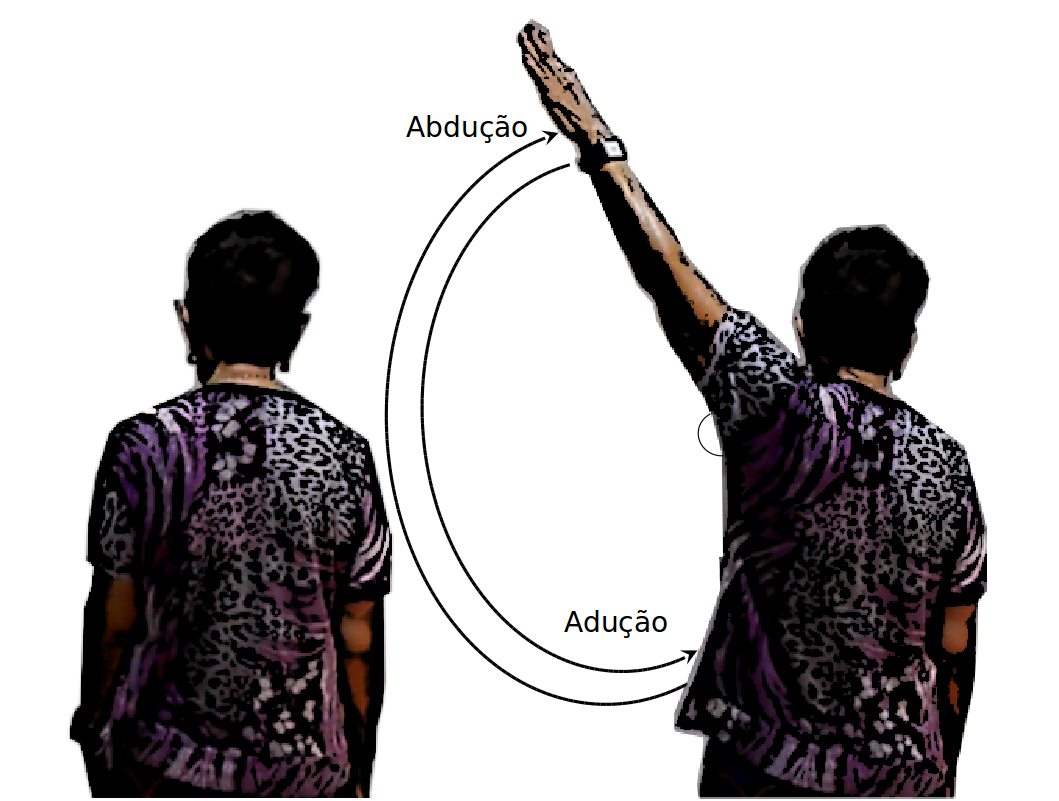
\includegraphics[scale=0.25]{./img/movaddcutctionartist2.png}
\caption{Movimentos de Abdução e Adução}
 \label{fig:movabducaomet}
\end{figure}

Durante a análise, foram comparados os Ângulos Relativos do Tronco e do Levantamento de Braços dos Indivíduos. As grandezas cinemáticas coletadas nesses estudo foram:
\begin{enumerate}
	\item A máxima amplitude atingida pelo movimento de abdução dos membros superiores;
	\item A velocidade angular de abdução dos membros superiores esquerdo e direito;
	\item A velocidade angular de adução dos membros superiores esquerdo e direito.
\end{enumerate}

Os dados coletados nesta fase resultaram na extração de características do movimento, incluindo: a amplitude do movimento dos braços do lado esquerdo e direito, e a velocidade angular dos movimentos de adução e abdução. Na Tabela~\ref{table:features} estão descritos os vetores de características:

\begin{table}[h]
\centering
\caption{Descrição do vetor de características extraído da coleta de dados.}
\label{table:features}
\begin{tabular}{|l|l|}
\hline
{\bf Característica}  & {\bf Descrição}                                       \\ \hline
MaxAmpEsquerdo     & Amplitude máxima do braço esquerdo. \\ \hline
MaxAmpDireito    & Amplitude máxima do braço direito. \\ \hline
AngVelAbdEsquerdo  & Velocidade angular do movimento de abdução do braço esquerdo. \\ \hline
AngVelAbdDireito & Velocidade angular do movimento de abdução do braço direito. \\ \hline
AngVelAdEsquerdo  & Velocidade angular do movimento de adução do braço esquerdo. \\ \hline
AngVelAdDireito & Velocidade angular do movimento de adução do braço direito. \\ \hline
\end{tabular}
\end{table}

\begin{figure}[!htb]
	\centering
	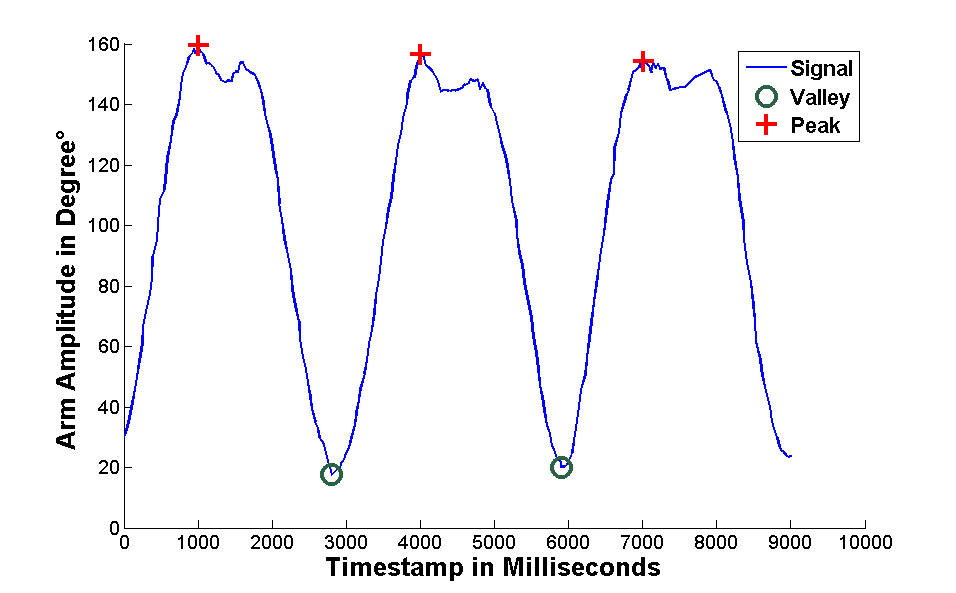
\includegraphics[width=1\textwidth]{img/signalamplitudepeakvaley-2.png}
	\caption{Exemplo do gráfico dos ângulos de adução e abdução dos braços em função do tempo}
	\label{fig:signalamplitudepeakvaley}
\end{figure}

A partir da extração das características do movimento, a próxima etapa da pesquisa foi classificar os dados de movimento e identificar a ocorrência do sintoma de bradicinesia. Por meio das teorias estatísticas de aprendizagem de máquina, foi realizado uma análise dos dados para aquisição de conhecimento utilizando aprendizagem supervisionada~\cite{kantardzic2011data}. 


\subsubsection{Relação Risco e Benefício da Pesquisa}
Os riscos inerentes podem decorrer da exposição de dados dos sujeitos da pesquisa. Isso pode acarretar em danos morais e/ou psicológicos. Logo, teve-se um cuidado de preservar a integridade física e psicológica dos sujeitos da pesquisa, garantindo assim a privacidade e a confidencialidade das informações.

Caso ocorresse algum constrangimento por parte do sujeito da pesquisa, ao não conseguir realizá-la, os pesquisadores prestariam total assistência, orientando-o adequadamente para prosseguir ou encerrar o procedimento. Os presentes riscos fazem jus aos benefícios que a pesquisa venha a trazer com a possibilidade de monitoramento dos sinais do~\ac{dp}. A identificação dos sinais motores e a classificação destes através do computador podem permitir avanços para um melhor acompanhamento da evolução da doença e possibilitar o monitoramento não invasivo dos pacientes.



\subsection{Aplicação do Método}
O propósito dessa classificação foi explorar a possibilidade de obter dados de saúde de forma contínua e não invasiva a partir de um sensor de captura de movimento usado em jogos eletrônicos (Ms-Kinnect). Durante a coleta dos dados foi indagado junto aos voluntários sua condição física e possíveis riscos e desconfortos que eles pudessem ter ao realizar o procedimento. 

Durante a pesquisa, partiu-se do princípio de que, através da análise do movimento de abdução e adução dos braços seria possível avaliar a biomecânica da amplitude do movimento dos braços e a sua velocidade angular. Então, por intermédio desses dados biomecânicos, seria possível identificar a ocorrência do sintoma de bradicinesia em indivíduos portadores do \ac{dp}.



\subsection{Resultados}
Conforme a abordagem~\ac{jogue-me} apresentada no Capítulo~\ref{chapter:abordagem_gahme}, os dados adquiridos foram processados, filtrados e postos em uma Máquina de Vetor de Suporte, para realizar a classificação entra as duas classes de dados. Para a classificação dos dados, foi utilizado um \textit{kernel} Linear (Seção~\ref{sec:svm_linear}), por ter obtido os melhores resultados dentre os demais \textit{kernels} (Polinomial, Radial e de MLP). O resultado do \textit{kernel} linear foi o mais expressivo entre os demais devido à separação linear ter dividido bem as duas classes. 

\subsubsection{Vetor Médio}
Nessa etapa da pesquisa, foi calculado o Vetor Médio (Seção~\ref{section:filtro_dados}), para entender melhor a diferença de movimento entre os sujeitos diagnosticados com \ac{dp} e os sujeitos sem o diagnóstico. Como pode ser visto na Figura~\ref{fig:vetor_medio_abducao}, a amplitude de movimento de um indivíduo diagnosticado com~\ac{dp} é bem menor do que a de um indivíduo sem o diagnóstico. Entretanto, por ter sido escalonado em 20 \textit{frames}, esse vetor médio perdeu a informação da velocidade do movimento.

\begin{figure}[!htbp]
 \centering
 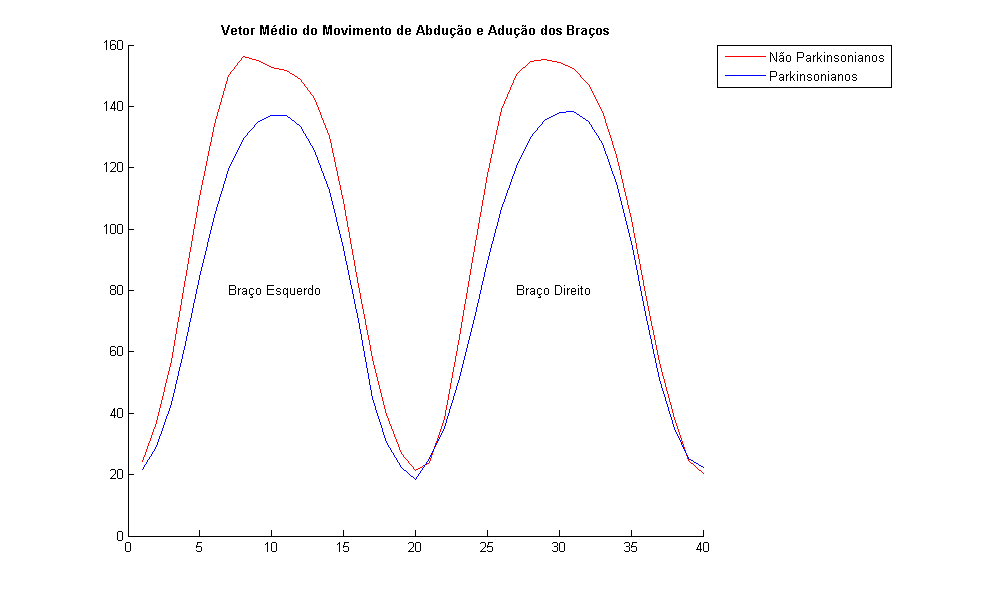
\includegraphics[scale=0.650]{./img/vetormedioaducao.png}
 \caption{Vetor Médio do Movimento de Abdução e Adução}
 \label{fig:vetor_medio_abducao}
\end{figure}


\subsubsection{Matriz de Confusão e Suas Métricas}
Para avaliar o resultado da classificação, será apresentada a \textbf{matriz de confusão}~\cite{kantardzic2011data}, que permite comparar os valores reais da classe com os valores obtidos no modelo de predição. 

A matriz de confusão para duas classes consiste numa matriz $2$\ x $2$\, contendo os \textit{Verdadeiros Positivos} (\textbf{TP}) e \textit{Verdadeiros Negativos} (\textbf{TN}), que são as classificações corretas. Os \textit{Falsos Negativos} (\textbf{FN}) contêm a predição incorreta de um valor que deveria ser positivo e os \textit{Falsos Positivos} (\textbf{FP}) contêm os valores positivos quando deveriam ser negativos, como pode ser visto na Tabela~\ref{table:descricaomatrizconfusao}.

% % Please remember to add \use{multirow} to your document preamble in order to suppor multirow cells
\begin{table}[!h]
\centering
\caption{Descrição da Matriz de Confusão}
\label{table:descricaomatrizconfusao}
\begin{tabular}{ll|l|l|}
\cline{3-4}
                                                                                                                & \textit{\textbf{}} & \multicolumn{2}{c|}{\textbf{Classe Preditiva}}                                                                                            \\ \cline{3-4} 
                                                                                                                &                    & \textbf{Parkinson}                                                   & \textbf{Controle}                                                  \\ \hline
\multicolumn{1}{|l|}{\multirow{2}{*}{\textit{\textbf{\begin{tabular}[c]{@{}l@{}}Classe\\ Atual\end{tabular}}}}} & \textbf{Parkinson} & \begin{tabular}[c]{@{}l@{}}Verdadeiros\\ Positivos (VP)\end{tabular} & \begin{tabular}[c]{@{}l@{}}Falsos\\ Negativos (FN)\end{tabular}    \\ \cline{2-4} 
\multicolumn{1}{|l|}{}                                                                                          & \textbf{Controle}  & \begin{tabular}[c]{@{}l@{}}Falsos\\ Positivos (FP)\end{tabular}      & \begin{tabular}[c]{@{}l@{}}Verdeiros\\ Negativos (VN)\end{tabular} \\ \hline
\end{tabular}
\end{table}



\subsection{Aprendizagem de Máquina (SVM)}

Para uma base de dados pequena, contendo apenas 30 indivíduos, o método de Validação Cruzada escolhido deve tentar maximizar o conjunto de treinamento para atingir um melhor resultado de teste. Por esse motivo, foi escolhida a validação cruzada \textit{leave-one-out}~\cite{kantardzic2011data}. 

O \textit{leave-one-out} é um método de validação cruzada \textit{k-fold} com o mesmo número de \textit{n} indivíduos. Logo, apenas um indivíduo será considerado teste e os demais serão de treinamento. Dessa maneira, não existe estratificação nos dados, tornando o processo determinístico e repetível com a mesma base de dados, o que reduz o problema de viés na seleção dos dados. Logo, a taxa de erro obtida da classificação é a taxa de erro do modelo para aquela base de dados. 

\subsubsection{Otimização dos Parâmetros da SVM - Método Grid-Search}

Para identificar os melhores parâmetros~\ac{svm}, foi aplicado o método~\textit{Grid-Search} ~\cite{gridsearchsvm2010} usando validação cruzada \textit{Leave-One-Out} (LOOCV)~\cite{kantardzic2011data}. Este método avalia a precisão do modelo previsto, evita o problema do superajuste na classificação binária e é um método prático para identificar os parâmetros SVM . Neste estudo, para reduzir a taxa de erro, nós aplicamos uma abordagem de \textit{minimax} visando maximizar a margem sobre os coeficientes hiperplano para obter uma classificação mais correta. Os valores dos parâmetros de pesquisa do \textit{grid-search} foram de: $C$ = [$2^{-5}$, ... ,$2^2$] e $\gamma$ = [$2^{-15}$, ... ,$2^3$ ], usando assim uma exponencial de base 2. Por meio deste método, foi possível identificar uma região em que o classificador possuía a melhor acurácia e a menor taxa de \textit{FpRate}. Após identificar essa região, realizamos uma busca mais detalhada com os seguintes parâmetros: $C$ = [0.25, 0.5, ... ,2.5]; e $\gamma$ = [1, 2,
 ...,10], como pode ser visto na Figura~\ref{fig:gridaccuracy}.


\begin{figure}[!h]
 \centering
  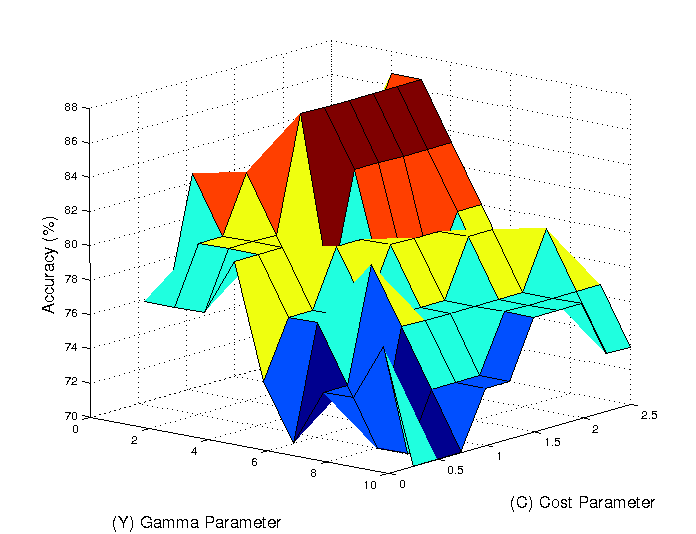
\includegraphics[scale=0.7]{./img/gridsearch.png} 
  \caption{\textit{Grid-Search} - Acurácia da Classificação}
 \label{fig:gridaccuracy}
\end{figure}

 
Como pode ser analisado na Figura~\ref{fig:gridaccuracy}, nós conseguimos uma classificação nos dados em que a pior predição obteve uma acurácia de 70,00\% e a melhor, de 86,67\%. Conseguimos também um baixo valor de \textit{FpRate}, com 6,67\% no melhor dos casos (Figura~\ref{fig:gridfprate}). Usando o método \textit{grid-search}, nós encontramos como melhor valor para os parâmetros: $C = 2$ and $\gamma = 3$. Como podemos analisar nos nossos resultados, por meio do método \textit{grid-search}, foi possível identificar parâmetros para o classificador~\ac{svm} com uma boa generalização e capaz de identificar a maior \textit{acurácia} e o menor \textit{FpRate}.


\begin{figure}[!h]
 \centering
 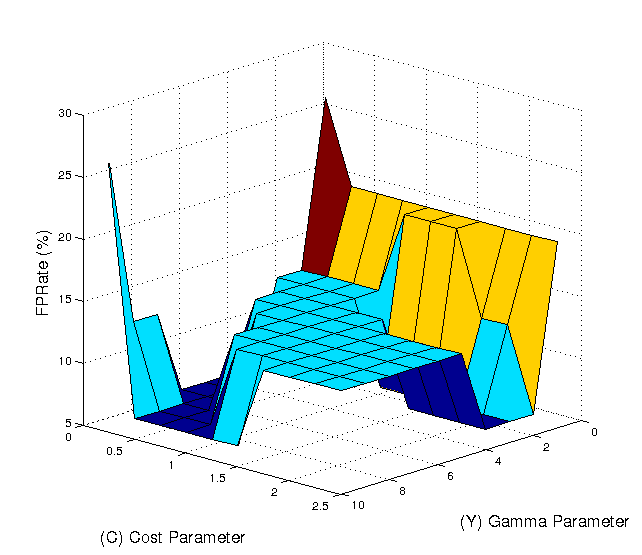
\includegraphics[scale=0.7]{./img/gridsearchfprate.png}
\caption{\textit{Grid-Search} - \textit{FpRate}}
 \label{fig:gridfprate}
\end{figure}


\subsubsection{Resultados Obtidos}\label{sec:resultado_obtido_svm}


A Matriz de Confusão obtida indica que existem três indivíduos classificados como ``Controle'', mas que possuem a doença (FN); no entanto, analisando as características do movimento dos indivíduos com~\ac{dp}, percebemos que eles apresentaram uma amplitude de movimento e uma velocidade angular bastante próximas dos indivíduos do Grupo Controle. Logo, estes não apresentam o sintoma de bradicinesia, o que pode indicar que o indivíduo esteja no início da doença, ou bem medicado, ou até mesmo não apresentar este sinal motor, o que corrobora com a sintomatologia do~\ac{dp}. 


\begin{table}[!htbp] 
\caption{Resultado da Matriz de Confusão SVM}
\label{table:resultadomatrizconfusaosvm}
\centering
\begin{tabular}{l|c|c|}
\cline{2-3}
\multicolumn{1}{c}{}                         & \multicolumn{2}{|c|}{\textit{\textbf{Classe Preditiva}}} \\ \cline{2-3} 
                                             & \textbf{Parkinson}      & \textbf{Controle}         \\ \hline
\multicolumn{1}{|l|}{\textbf{Parkinson}} & 12       & 3           \\ \hline
\multicolumn{1}{|l|}{\textbf{Controle}}     & 1           & 14     \\ \hline
\end{tabular}

\end{table}

O sinal da bradicinesia presente no~\ac{dp} foi quantificado pela amplitude do movimento de abdução dos braços e sua respectiva velocidade angular. Na análise destes sinais, foi possível extrair os vetores de características para a classificação dos dados~\cite{kantardzic2011data}. Na Tabela~\ref{table:amplitude}, podemos demonstrar a severidade do sinal motor causado pela bradicinesia, em que o Grupo com~\ac{dp} apresentou amplitudes bem menores ante os indivíduos do Grupo Controle. Notamos também que o indivíduo ``Controle 10'' apresentou uma amplitude muito semelhante aos do Grupo com~\ac{dp}. Neste caso, nós identificamos que ele apresentava um problema motor e isso ocasionou uma classificação incorreta por parte da~\ac{svm}. Além disso, 3 indivíduos do Grupo com~\ac{dp} (3,8 e 12) não apresentavam o sinal da bradicinesia durante a coleta. Nestes casos, podemos assumir que eles não possuem a bradicinesia, ou o sinal estava suprimido pela medicação.


\begin{table}[!htp]
\centering
\caption{Média da Amplitude do Movimento de Abdução do Braço}
\label{table:amplitude}
\begin{tabular}{|l|l|l|l|}
\hline
\textbf{Indivíduo} & \textbf{\begin{tabular}[c]{@{}l@{}}Média da\\ Amplitude \\ Braço Esquerdo(º)\end{tabular}} & \textbf{\begin{tabular}[c]{@{}l@{}}Média da\\ Amplitude\\ Braço Direito(º) \end{tabular}} & \textbf{\begin{tabular}[c]{@{}l@{}}Classe\\ Preditiva\end{tabular}} \\ \hline
Controle 1         & \multicolumn{1}{r|}{153.62}                                                          & \multicolumn{1}{r|}{151.14}                                                          & Controle                                                            \\ \hline
Controle 2         & \multicolumn{1}{r|}{165.31}                                                          & \multicolumn{1}{r|}{151.84}                                                          & Controle                                                            \\ \hline
Controle 3         & \multicolumn{1}{r|}{155.44}                                                          & \multicolumn{1}{r|}{163.31}                                                          & Controle                                                            \\ \hline
Controle 4         & \multicolumn{1}{r|}{169.12}                                                          & \multicolumn{1}{r|}{169.39}                                                          & Controle                                                            \\ \hline
Controle 5         & \multicolumn{1}{r|}{157.20}                                                          & \multicolumn{1}{r|}{162.72}                                                          & Controle                                                            \\ \hline
Controle 6         & \multicolumn{1}{r|}{162.99}                                                          & \multicolumn{1}{r|}{167.25}                                                          & Controle                                                            \\ \hline
Controle 7         & \multicolumn{1}{r|}{166.90}                                                          & \multicolumn{1}{r|}{166.93}                                                          & Controle                                                            \\ \hline
Controle 8         & \multicolumn{1}{r|}{154.68}                                                          & \multicolumn{1}{r|}{159.13}                                                          & Controle                                                            \\ \hline
Controle 9         & \multicolumn{1}{r|}{162.31}                                                          & \multicolumn{1}{r|}{158.17}                                                          & Controle                                                            \\ \hline
Controle 10         & \multicolumn{1}{r|}{135.22}                                                          & \multicolumn{1}{r|}{131.85}                                                          & \textbf{Parkinson}                                                            \\ \hline
Controle 11         & \multicolumn{1}{r|}{162.13}                                                          & \multicolumn{1}{r|}{167.61}                                                          & Controle                                                            \\ \hline
Controle 12         & \multicolumn{1}{r|}{161.69}                                                          & \multicolumn{1}{r|}{166.78}                                                          & Controle                                                            \\ \hline
Controle 13         & \multicolumn{1}{r|}{160.47}                                                          & \multicolumn{1}{r|}{155.05}                                                          & Controle                                                            \\ \hline
Controle 14         & \multicolumn{1}{r|}{174.37}                                                          & \multicolumn{1}{r|}{167.66}                                                          & Controle                                                            \\ \hline
Controle 15         & \multicolumn{1}{r|}{155.08}                                                          & \multicolumn{1}{r|}{167.83}                                                          & Controle                                                            \\ \hline
Parkinson 1         & \multicolumn{1}{r|}{125.80}                                                          & \multicolumn{1}{r|}{119.73}                                                          & Parkinson                                                            \\ \hline
Parkinson 2         & \multicolumn{1}{r|}{131.28}                                                          & \multicolumn{1}{r|}{123.49}                                                          & Parkinson                                                            \\ \hline
Parkinson 3         & \multicolumn{1}{r|}{156.66}                                                          & \multicolumn{1}{r|}{149.46}                                                          & \textbf{Controle}                                                            \\ \hline
Parkinson 4         & \multicolumn{1}{r|}{139.90}                                                          & \multicolumn{1}{r|}{142.83}                                                          & Parkinson                                                            \\ \hline
Parkinson 5         & \multicolumn{1}{r|}{147.37}                                                          & \multicolumn{1}{r|}{153.13}                                                          & Parkinson         \\ \hline
Parkinson 6         & \multicolumn{1}{r|}{115.32}                                                          & \multicolumn{1}{r|}{123.56}                                                          & Parkinson                                                            \\ \hline
Parkinson 7         & \multicolumn{1}{r|}{129.75}                                                          & \multicolumn{1}{r|}{133.04}                                                          & Parkinson                                                            \\ \hline
Parkinson 8         & \multicolumn{1}{r|}{166.62}                                                          & \multicolumn{1}{r|}{165.63}                                                          & \textbf{Controle}                                                            \\ \hline
Parkinson 9         & \multicolumn{1}{r|}{143.95}                                                          & \multicolumn{1}{r|}{140.45}                                                          & Parkinson                                                            \\ \hline
Parkinson 10         & \multicolumn{1}{r|}{136.86}                                                          & \multicolumn{1}{r|}{151.03}                                                          & Parkinson                                                            \\ \hline
Parkinson 11         & \multicolumn{1}{r|}{156.87}                                                          & \multicolumn{1}{r|}{142.93}                                                          & Parkinson                                                            \\ \hline
Parkinson 12         & \multicolumn{1}{r|}{166.59}                                                          & \multicolumn{1}{r|}{157.81}                                                          & \textbf{Controle}                                                            \\ \hline
Parkinson 13         & \multicolumn{1}{r|}{147.99}                                                          & \multicolumn{1}{r|}{142.02}                                                          & Parkinson                                                            \\ \hline
Parkinson 14         & \multicolumn{1}{r|}{141.95}                                                          & \multicolumn{1}{r|}{150.60}                                                          & Parkinson                                                            \\ \hline
Parkinson 15         & \multicolumn{1}{r|}{125.69}                                                          & \multicolumn{1}{r|}{140.62}                                                          & Parkinson                                                            
\\ \hline
\end{tabular}
\end{table}

Para demonstrar a avaliação do modelo de forma quantitativa, usou-se um conjunto de métricas derivadas da matriz de confusão~\cite{kantardzic2011data}.
 \begin{description}
 	\item [\textit{TpRate}] taxa de acerto obtido: $ TpRate = TP/P $\ ;
 	\item [\textit{FpRate}]: taxa de falso alarme obtido: $ FpRate = FP/N $\ ;
 	\item [\textit{Precision}]: taxa de acerto de uma instância em determinada classe: $ Precision =  TP/(TP +FP) $\ ;
 	\item [\textit{Accuracy}]: taxa de acerto de todo o classificador: $ Accuracy = (TP+TN)/(P+N) $\ ;
 	\item [\textit{F-Measure}]: análise de classificador binário que mede a acurácia do teste, considerando a média harmônica da taxa de \textit{precision} e do \textit{tp rate}: $ F-Measure = 2 * (Precision * TpRate)/(Precision + TpRate) $\ .
 \end{description}



\begin{table}[!htbp]
\label{table:metricasmatrizconfusao}
\caption{Métricas da Matriz de Confusão}
\centering
\begin{tabular}{|l|r|}
\hline
\multicolumn{2}{|l|}{\textbf{Métricas}} \\ \hline
\textbf{TpRate}                    & 80,00$\%$\                 \\ \hline
\textbf{FpRate}                    & 6,67$\%$\                \\ \hline
\textbf{Precision}                 & 92,31$\%$\                \\ \hline
\textbf{Accuracy}                  & 86,67$\%$\                \\ \hline
\textbf{F-Measure}                 & 85,71$\%$\                \\ \hline
\end{tabular}
\end{table}








\section{ETAPA 3 - Avaliação Da Aceitação Da Abordagem Junto aos Pacientes com~\ac{dp} Utilizando \textit{Goal Question Metric}}\label{gqm_usuarios}


Com o objetivo de averiguar a possibilidade de integrar o monitoramento da saúde do jogador através de jogos eletrônicos à sua rotina diária, foi utilizada a abordagem \textit{Goal, Question, Metric} (GQM)~\cite{van1999goal}. Essa abordagem é um paradigma de pesquisa utilizado na Engenharia de Software para medição de processos de software e melhoria contínua dos produtos ~\cite{saraiva2006,elicquest05}. A qualidade do produto de software~\cite{saraiva2006} pode ser compreendida como a adequação a um conjunto de características atingidas em maior ou menor grau para que o produto final venha atender as necessidades do usuário, identificadas na fase de elicitação de requisitos~\cite{elicquest05}.

O~\ac{gqm} é um paradigma de avaliação orientado por metas e tem como componentes elementares: objetivos, questionamentos e métricas~\cite{saraiva2006}. Nesse paradigma de pesquisa é definido um objetivo principal, em que as perguntas são refinadas para que se venha extrair as métricas da pesquisa. De posse das respostas baseadas em métricas, estas são comparadas com o objetivo da pesquisa no intuito de identificar se ele foi alcançado. Logo, o paradigma~\ac{gqm} busca definir métricas partindo de uma perspectiva de ``de cima para baixo'', e analisa, interpreta e mensura dados de maneira ``de baixo para cima'', como pode ser graficamente visualizado na Figura~\ref{fig:gqm} ~\cite{van1999goal}. 

\begin{figure}[!htbp]
 \centering
 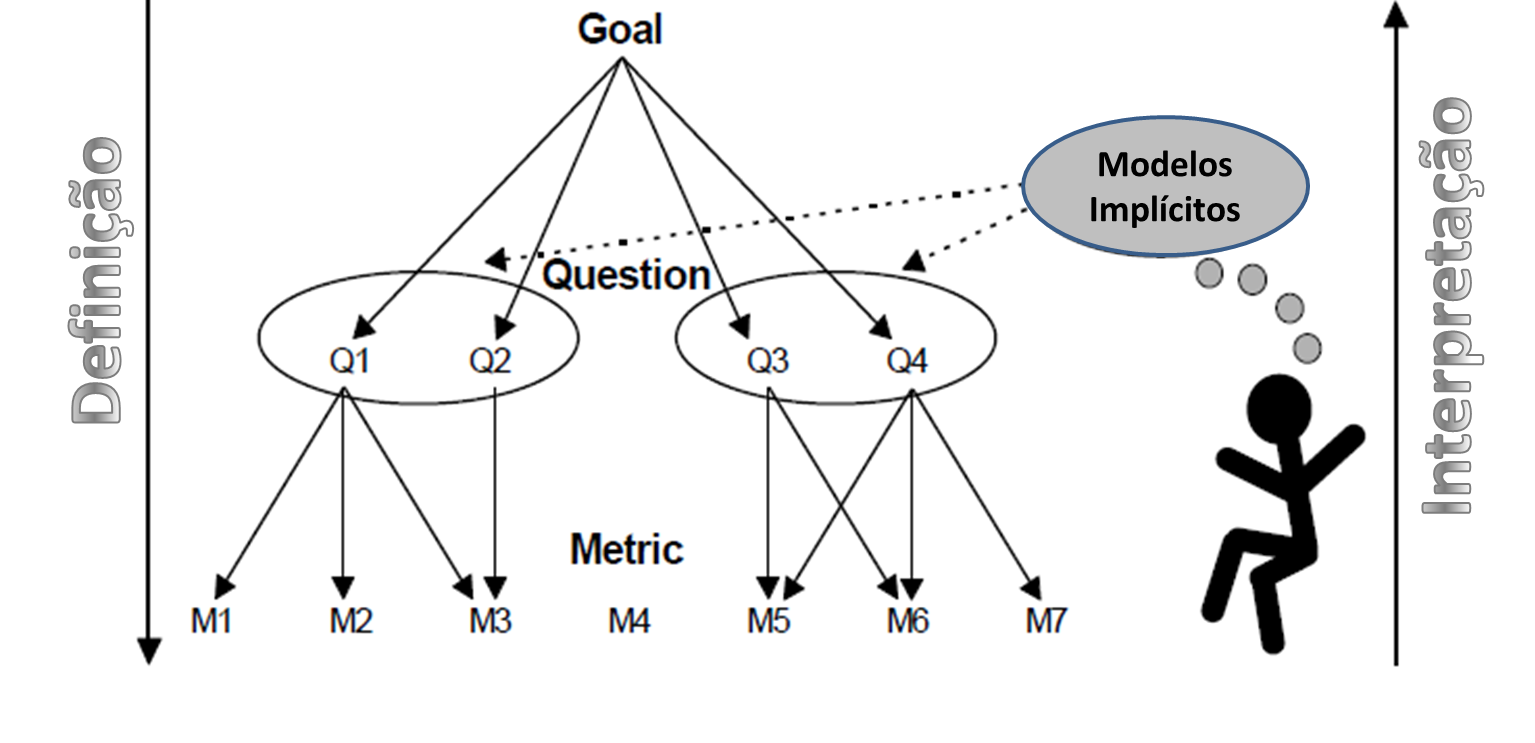
\includegraphics[scale=0.50]{./img/gqm.png}
 \caption[O Paradigma GQM \copyright]{O Paradigma GQM \copyright~\cite{van1999goal}}
 \label{fig:gqm}
\end{figure}

Segundo Saraiva ~\cite{saraiva2006}, numa análise da aplicação do método de ~\ac{gqm} para o contexto de avaliação de usabilidade de software, os componentes elementares do paradigma ~\ac{gqm} são:

\begin{itemize}
	\item \textbf{Objetivo}: Sua definição envolve o propósito da avaliação, o que deve ser avaliado, a perspectiva e o ambiente proposto.
	\item \textbf{Questão}: A questão anuncia a necessidade de se obter informações em linguagem natural, podendo formular uma ou mais questões para cada categoria. Logo, sua resposta deve estar condicionada ao objetivo proposto.
	\item \textbf{Métrica}: Sua função é especificar os dados que se deseja obter durante as avaliações em termos quantitativos, podendo ter mais de uma métrica para cada questão.	
\end{itemize}

Baseado nos componentes elementares do paradigma, foi elaborado um questionário~\ac{gqm} (Apêndice~\ref{apend:gqm}), com o objetivo principal de avaliar a possibilidade de monitorar dados motores, de forma não invasiva e integrada à rotina diária dos usuários. Para elaboração de métricas para atingir esse objetivo foram formuladas duas questões de pesquisa, com o intuito de avaliar:
\begin{enumerate}
	\item se o usuário integraria a abordagem~\ac{jogue-me} à sua rotina diária;
	\item se a segurança com a integridade física está de acordo com a faixa etária do usuário.
\end{enumerate}

O questionário consistiu de um conjunto de 10 questões de resposta fechada (quantitativa) ~\cite{elicquest05}, e o entrevistado teve de escolher uma resposta dentre as alternativas dadas. Esse método foi escolhido para contribuir por uma maior uniformidade nas respostas e, consequentemente, facilitar sua análise. Porém, este método impede a expressão das opiniões dos entrevistados~\cite{elicquest05}. 


\subsection{Aplicação do Método}
Nessa etapa da pesquisa foram avaliados 30 sujeitos, dos seguintes locais: Hospital Universitário da UFAL, Fundação Pestalozzi e clínica de Fisioterapia do CESMAC. Os usuários foram selecionados para jogar o \emph{Catch the Spheres} (Seção ~\ref{jogo_catch}), testaram e responderam o questionário para verificar a aceitabilidade da abordagem. 


\subsection{Resultados}
Os resultados do questionário são apresentados na Tabela~\ref{table:resultados_gqm}, contendo as respostas binárias ``Sim/Não'', e nas Figuras~\ref{fig:question1}, \ref{fig:question3} e \ref{fig:question10}, com a reposta das perguntas de questões com múltipla escolha.

\textit{Questão 1 - O usuário poderia integrar a abordagem~\ac{jogue-me} à sua rotina diária ?}: os 24 usuários deram as seguintes respostas nas Métricas (1.1, 1.2, 1.3,1.4,1.5 e 1.6): 75\% dos usuário atribuíram ao menos nota 4 (de 1 a 5) ao grau de diversão do jogo; 91,67\% sentiram-se motivados com o jogo; 58\% dos usuários jogariam 3 vezes por semana, 25\% jogariam todos os dias e apenas 17\% jogariam uma vez por semana. 

Então, tem-se um percentual de 83\% de usuários que poderiam integrar o monitoramento motor a sua rotina; 91,67\% consideraram o jogo simples e de fácil entendimento, e isso permite o uso de um maior número de usuários. Uma métrica desfavorável foi que apenas 41,67\% dos usuários possuem o costume de usar jogos casuais em casa. Mas, devido à expectativa de melhora do estado de saúde, 75\% dos usuários responderam que agregariam o jogo a sua rotina diária.

\textit{Questão 2 - A segurança com a integridade física está de acordo com a faixa etária do usuário
?}: nesta questão, percebe-se uma grande preocupação dos usuários quanto ao risco de quedas. Inicialmente, a pesquisa seria destinada para o movimento de braços e pernas. Devido aos riscos, foi modificada para a movimentação somente dos braços, reduzindo a preocupação dos usuários. Mesmo assim, as métricas obtidas demonstraram que o jogo é seguro para crianças e adultos. No caso dos idosos, 75\% dos usuários consideraram o jogo seguro para essa faixa etária, muito embora os mesmos usuários classificaram o jogo com a faixa etária ``livre'', com 88\% de ocorrência.

% Please remember to add \use{multirow} to your document preamble in order to suppor multirow cells
\begin{table}[h]
\caption{Métricas Avaliadas do \textit{GQM}}
\centering
\begin{tabular}{|p{10cm}|p{1.2cm}|p{1.2cm}|}
\hline
\textbf{Métrica} & \textbf{Sim} & \textbf{Não} \\ \hline
1.2: O jogo traz motivação ao usuário? & 91,67\% & 8,33\% \\ \hline
1.4: O usuário considera o jogo simples, sem muitas regras e de fácil entendimento? Ele pode ser aplicado em diferentes idades? & 91,67\% & 8,33\% \\ \hline
1.5: O usuário tem o costume de jogar esses jogos casuais em casa? & 41,67\% & 58,33\% \\ \hline
1.6: O usuário agregaria um jogo desse estilo em sua rotina diária? & 75\% & 25\% \\ \hline
2.1: Uma criança estaria segura jogando esse jogo, ao efetuar os movimentos dos braços? & 100\% & 0\% \\ \hline
2.2: Um adulto estaria seguro ao jogar esse jogo, ao efetuar os movimentos dos braços? & 100\% & 0\% \\ \hline
2.3: Um idoso estaria seguro ao jogar esse jogo, ao efetuar os movimentos dos braços? & 75\% & 25\% \\ \hline
\end{tabular}
\label{table:resultados_gqm}
\end{table}


\begin{figure}[!htb]
     \centering
     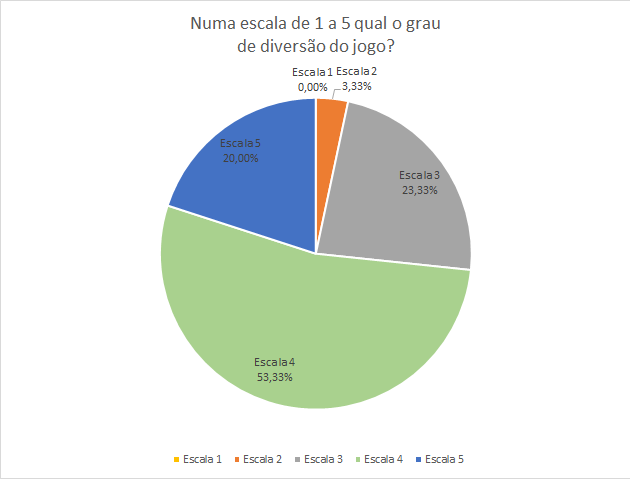
\includegraphics[scale=0.7]{./img/chart_1-.png}
     \caption{Resultado da Pergunta 1}
     \label{fig:question1}
\end{figure}


\begin{figure}[!htb]
     \centering
     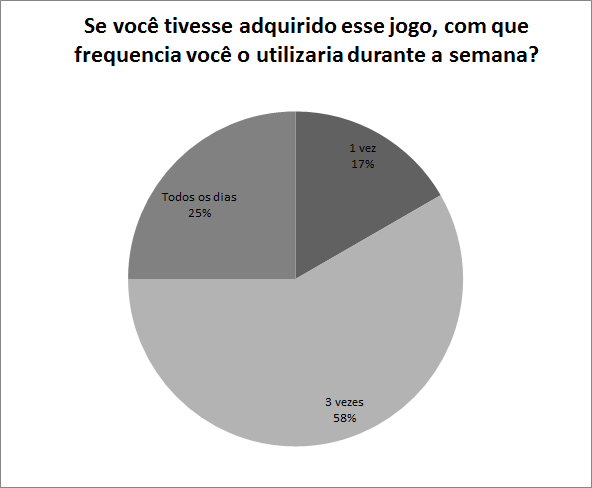
\includegraphics[scale=0.7]{./img/chart_3-.png}
     \caption{Resultado da Pergunta 3}
     \label{fig:question3}
\end{figure}


\begin{figure}[!htb]
     \centering
     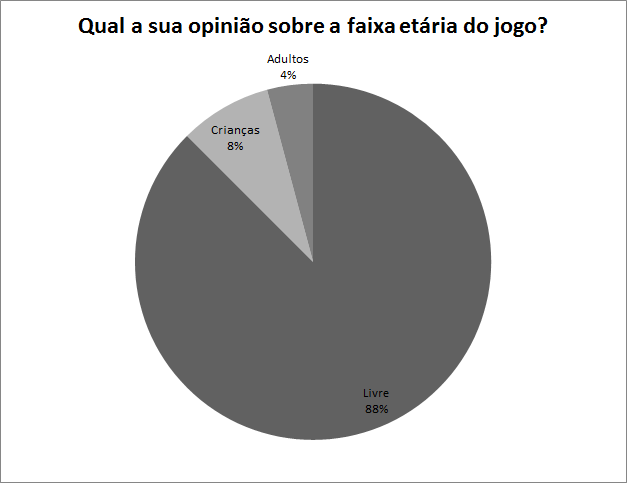
\includegraphics[scale=0.7]{./img/chart_10-.png}
     \caption{Resultado da Pergunta 10}
     \label{fig:question10}
\end{figure}
\FloatBarrier

De acordo com o resultado da avaliação dos usuários usando~\ac{gqm}, identificamos que a abordagem de um~\ac{sms} dos sinais motores usando jogos, como interface de entrada de dados, conseguiu motivar o usuário  a fornecer sinais motores e permite o acompanhar o tratamento a partir dos dados biomecânicos adquiridos. Logo, conseguimos atingir o principal objetivo da tese, ao demonstrar o monitoramento dos pacientes com~\ac{dp} de uma maneira não invasiva e no conforto de seus lares.






